\chapter{\nmu Resultados} % (fold)
\label{cha:resultados}
% http://pypi-ranking.info/alltime
% http://popcon.ubuntu.com/
% http://popcon.debian.com/

% entre os 30 mais
% ncurses-base
% sed
% bash
% tar
% perl-base
% mount
% gzip


\begin{table}[htbp]
\caption{Comparação de resultados}
\resizebox{\columnwidth}{!}{%
\begin{tabular}[c]{clccccc}
\toprule
\multicolumn{ 2}{c}{\textbf{Pacote}} & \textbf{apt} & \textbf{apt-cache} & \textbf{Exact Match} & \textbf{Levenshtein} & \textbf{Smith-Waterman} \\ \midrule
\multicolumn{ 1}{c}{} & \textit{posição} & 27 & 3 & 1 & 1 & 1 \\ 
\multicolumn{ 1}{c}{\textbf{ncurses-base}} & \textit{dimensão} & 37 & 37 & 1 & $-$ & $-$ \\ 
\multicolumn{ 1}{c}{} & \textit{tempo [s]} & 0.874 & 0.349 & 1.146 & 9.539 & 52.212 \\ \hline
\multicolumn{ 1}{c}{} & \textit{posição} & *** & *** & 48 & 1 & 1 \\ 
\multicolumn{ 1}{c}{\textbf{sed}} & \textit{dimensão} & *** & *** & * & $-$ & $-$ \\ 
\multicolumn{ 1}{l}{} & \textit{tempo [s]} & 0.968 & 0.358 & 1.102 & 9.125 & 16.421 \\ \hline
\multicolumn{ 1}{c}{} & \textit{posição} & 6 & 1 & 1 & 2 & 1 \\ 
\multicolumn{ 1}{c}{\textbf{bash}} & \textit{dimensão} & * & * & 13 & $-$ & $-$ \\ 
\multicolumn{ 1}{c}{} & \textit{tempo [s]} & 0.901 & 0.335 & 1.142 & 9.343 & 20.518 \\ \hline
\multicolumn{ 1}{c}{} & \textit{posição} & *** & * & * & 2 & 1 \\ 
\multicolumn{ 1}{c}{\textbf{tar}} & \textit{dimensão} & * & * & * & $-$ & $-$ \\ 
\multicolumn{ 1}{c}{} & \textit{tempo [s]} & 0.923 & 0.373 & 1.137 & 9.028 & 16.02 \\ \hline
\multicolumn{ 1}{c}{} & \textit{posição} & 13 & 2 & 1 & 1 & 1 \\ 
\multicolumn{ 1}{c}{\textbf{perl-base}} & \textit{dimensão} & 16 & 16 & 2 & $-$ & $-$ \\ 
\multicolumn{ 1}{c}{} & \textit{tempo [s]} & 0.936 & 0.311 & 1.116 & 9.36 & 41.548 \\ \hline
\multicolumn{ 1}{c}{} & \textit{posição} & * & 52 & 23 & 1 & 1 \\ 
\multicolumn{ 1}{c}{\textbf{mount}} & \textit{dimensão} & * & * & 37 & $-$ & $-$ \\ 
\multicolumn{ 1}{c}{} & \textit{tempo [s]} & 0.895 & 0.338 & 1.121 & 9.082 & 24.848 \\ \hline
\multicolumn{ 1}{c}{} & \textit{posição} & 23 & 5 & 1 & 1 & 1 \\ 
\multicolumn{ 1}{c}{\textbf{gzip}} & \textit{dimensão} & * & * & 5 & $-$ & $-$ \\ 
\multicolumn{ 1}{c}{} & \textit{tempo [s]} & 0.876 & 0.324 & 1.103 & 9.482 & 20.163 \\ \bottomrule
\end{tabular}
}

% \subcaption{Fonte: \href{http://popcon.ubuntu.com/}{Popcorn-Ubuntu}\protect\footnotemark}
\label{tab:comparacao}
\begin{description}
	\tiny
	%\item [Legenda]
	\item [*] Acima de 100 pacotes.
	\item [**] Acima de 1000 pacotes.
	\item [***] Acima de 10000 pacotes.
	\item [$-$] Quantidade desconsiderada
\end{description}

\end{table}
% \footnotetext{\label{tab:comparacao_footnote}Ordenado pelo número de pessoas que instalaram o pacote.}


Tomados os devidos valores, foi montada então a \autoref{tab:comparacao} com 7 (sete) dentre os 30 (trinta) pacotes mais instalados segundo o \href{http://popcon.ubuntu.com/}{Popcorn-Ubuntu}. Para uma melhor apresentação dos dados, valores acima de $100$ foram desconsiderados e as opções de uso de \textit{pool de threads} não foram utilizadas.

O que  podemos observar  segundo a \autoref{tab:comparacao} é um certa deficiência em apresentar os pacotes realmente desejados no topo da lista de possibilidades quando se trata dos métodos padrões de busca, {\code apt} e {\code apt-cache}. Com a busca realizada no {\code apt}, a busca pelo pacote {\code bash} foi a mais felizarda, posicionando o pacote desejado na $6ª$ posição, porém teve resultados terríveis quando observado a busca pelos pacotes {\code sed} e {\code tar}, onde ambos apareciam na lista, após a $10000ª$ posição


Devido o formato como o os prototipos de \textit{Levenshtein} e \textit{Smith} estão escritos, é possível se imprimir uma comparação com toda a lista de pacotes disponíveis na \textit{cache}. Assim, apenas os $50$ primeiros pacotes eram impressos para verificação. Assim, a linha \textit{dimensão} da tabela para estes algoritmos foi desconsiderada.

\begin{figure}[h]
  \centering
	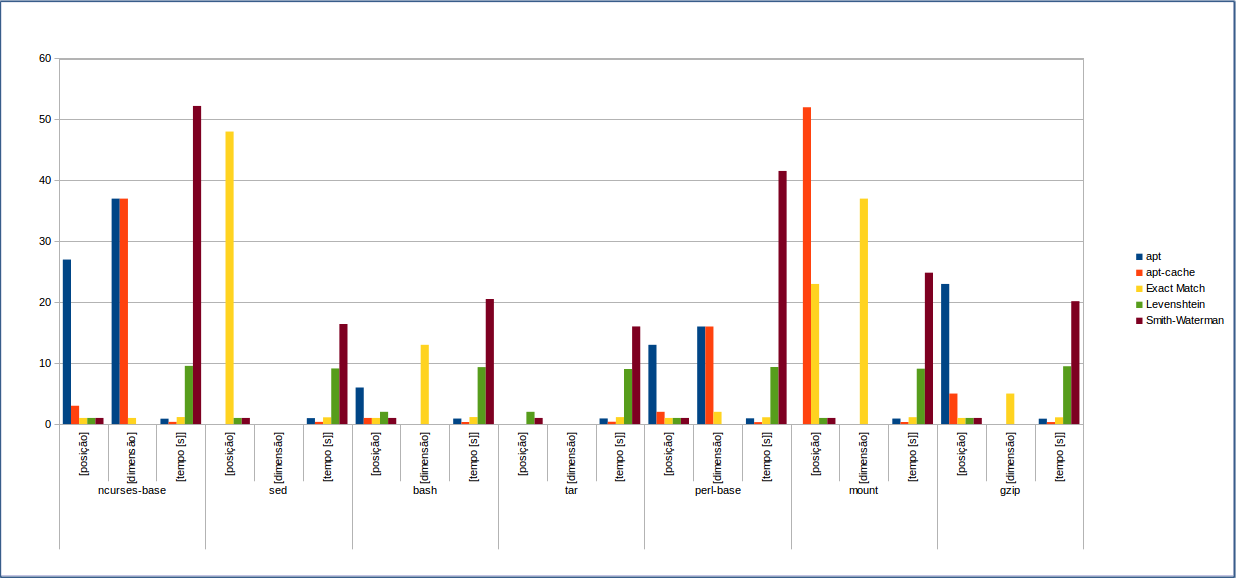
\includegraphics[width=\textwidth,angle=0]{figuras/grafico}
  \caption{Amostra de comparação dos resultados}
  \label{fig:figuras_grafico}
\end{figure}

A \autoref{fig:figuras_grafico} apresenta um gráfico representativo da \autoref{tab:comparacao} com a supressão dos valores acima de 100  para melhor visualização.

O que podemos observar deste trabalho é um resultado proporcional ao que se esperava, de quanto maior o trabalho ou a complexidade do algoritmo para ordenação, maior será o tempo necessário para a pesquisa, porém melhor serão os resultados obtidos na ordenação.

Podemos compreender também por que o {\code apt-cache} é mais utilizado que o próprio {\code apt}. Por ordenar todos os pacotes que retornam da pesquisa sem considerar a \textit{string} de entrada, o {\code apt} em momento algum apresentou resultados melhores que o {\code apt-cache} e ainda gastava um tempo de resposta aproximadamente 3 vezes maior. Se o algoritmo de busca atual do {\code apt} fosse substituído pelo modelo do \textit{Exact Match}, ele apresentaria resultados melhores que o do {\code apt-cache} gastando cerca de $300$ ms a mais que gasta atualmente. Porém, ambos algoritmos deixariam a desejar na apresentação de pacotes quando ocorresse uma escrita errada do pacote, visto que nenhum deles esta voltado para prever erros ortográficos.

Uma situação ideal seria obter os resultados alcançados com o algoritmo de \textit{Smith-Waterman} com o tempo de resposta que o {\code apt-cache} leva atualmente. Porém a realidade é que o tempo gasto pelo algoritmo de \textit{Smith-Waterman} é hoje impraticável, visto que quanto maior o tamanho do nome do pacote, maior é o tempo de resposta, levando a gastar quase 1 (um) minuto para uma busca pelo pacote {\code ncurses-base}. Porém o tempo gasto pelo algoritmo de 
\textit{Levenshtein} se mostra valido para futuros estudos de otimização e inclusão nas rotinas de busca quando retornar poucos pacotes ou nenhum pacote, considerando assim que possa ter acontecido um erro de digitação. Neste caso seria importante apresentar ao usuário que existe a possibilidade de escrita incorreta de pacote antes da apresentação dos resultados.


\begin{table}[htbp]
\caption{Comparação de resultados com entradas contendo erros de ortografia}
\resizebox{\columnwidth}{!}{%
\begin{tabular}[c]{clccccc}
\toprule
\multicolumn{ 2}{c}{\textbf{Pacote}} & \textbf{apt} & \textbf{apt-cache} & \textbf{Exact Match} & \textbf{Levenshtein} & \textbf{Smith-Waterman} \\ \midrule
\multicolumn{ 1}{c}{\textbf{pitom-dev}} & \textit{posição} & 0 & 0 & 0 & 15 & 11 \\ 
\multicolumn{ 1}{c}{\textbf{[python-dev]}} & \textit{dimensão} & 0 & 0 & 0 & $-$ & $-$ \\ 
\multicolumn{ 1}{l}{} & \textit{tempo [s]} & 0.894 & 0.325 & 1.1 & 17.443 & 45.148 \\ \hline
\multicolumn{ 1}{c}{\textbf{gyth-core }} & \textit{posição} & 0 & 0 & 0 & 1 & 16 \\ 
\multicolumn{ 1}{c}{\textbf{[git-core]}} & \textit{dimensão} & 0 & 0 & 0 & $-$ & $-$ \\ 
\multicolumn{ 1}{l}{} & \textit{tempo [s]} & 0.872 & 0.316 & 1.124 & 17.757 & 40.694 \\ \hline
\multicolumn{ 1}{c}{\textbf{libbesh}} & \textit{posição} & 0 & 0 & 0 & 4 & 2 \\ 
\multicolumn{ 1}{c}{\textbf{[libbash]}} & \textit{dimensão} & 0 & 0 & 0 & $-$ & $-$ \\ 
\multicolumn{ 1}{l}{} & \textit{tempo [s]} & 0.816 & 0.331 & 1.121 & 17.481 & 32.686 \\ \hline
\multicolumn{ 1}{c}{\textbf{g-zip }} & \textit{posição} & 0 & 0 & 0 & 1 & 1 \\ 
\multicolumn{ 1}{c}{\textbf{[gzip]}} & \textit{dimensão} & 0 & 0 & 0 & $-$ & $-$ \\ 
\multicolumn{ 1}{l}{} & \textit{tempo [s]} & 0.881 & 0.312 & 1.118 & 17.237 & 24.224 \\ \bottomrule
\end{tabular}
}
\label{tab:comparacao2}
\begin{description}
	\tiny
	%\item [Legenda]
	% \item [0] Sem resultados.
	\item [$-$] Quantidade desconsiderada
\end{description}
\end{table}

Também foi verificado uma busca apenas com a escrita errada de pacotes para simular o desconhecimento do nome do pacote pelo usuário, fazendo com que fosse influenciado apenas pela fonética do pacote, tanto para simular um casual erro de digitação que se passa desapercebido. A \autoref{tab:comparacao2} apresenta estes resultados para alguns pacotes - contendo entre colchetes o nome correto do pacote. Como já é de conhecimento, as aplicações {\code apt} e {\code apt-cache} não possuem algoritmo que possa buscar por pacotes com o nome semelhante ao digitado quando não há resultados. Desta forma, as saídas para estas aplicações foram nulas devido a não existir um pacote com o nome fornecido na busca. Por fazer um processo de busca exata, o algoritmo de nome exato também não conseguiu encontrar nenhum pacote para apresentar de resultado quando era fornecido um nome inexistente dentre os pacotes disponíveis. 

Para os algoritmos de \textit{Levenshtein} e \textit{Smith-Waterman} os resultados já são bem diferentes, já  que ambos apresentam resultados baseados em aproximação de nomes. O algoritmo de \textit{Levenshtein} conseguiu manter três dos quatro testes entre os cinco primeiros resultados. Já o de \textit{Smith-Waterman} conseguiu manter apenas em metade dos casos o pacote desejado entre os cinco primeiros - mesmo tendo um melhor resultado na procura pelo pacote {\code pithom-dev} onde foram inseridos dois erros ortográficos.

O provável motivo pelo qual os resultados no algoritmo de \textit{Levenshtein} tenha se saído melhor nestes teste é em decorrer do fato de apenas este prototipo estava preparado para melhor classificar os pacotes que tivessem alguns prefixos ou sufixos predefinidos (\textit{lib}, \textit{-core}, \textit{-dev}, \textit{-commom} e \textit{-devel}).
Todavia, podemos observar um aumento acentuado no tempo necessário para a realização da busca no algoritmo de \textit{Levenshtein} enquanto no algoritmo de \textit{Smith-Waterman} se manteve pouco acima da média de tempo necessário ($35.688$ segundos contra $27.39$ segundos).